\section{Convex Learning Problems}
\frame{\tableofcontents[currentsection, hideothersubsections]}

% In general, a convex learning problem is a problem whose hypothesis class is a
% convex set, and whose loss function is a convex function for each example.

\begin{frame}
\frametitle{Convex Learning Problems: Intro}

Recall, we have:
\begin{itemize}
    \item a set of examples $\mathcal{Z} = \mathcal{X} \times \mathcal{Y}$
    \item a hypothesis class $\mathcal{H}$, which can be an arbitrary set,\\
    for now consider: $ \mathcal{H} \subset R^d$, i.e.
    every hypothesis is some real-valued vector;
    thus, denote a hypothesis in $\mathcal{H}$ by $\mathbf{w}$
    \item a loss function $\mathcal{L}: \mathcal{H} \times \mathcal{Z} \mapsto \mathbb{R_{+}}$
\end{itemize}

\begin{figure}
    \centering
    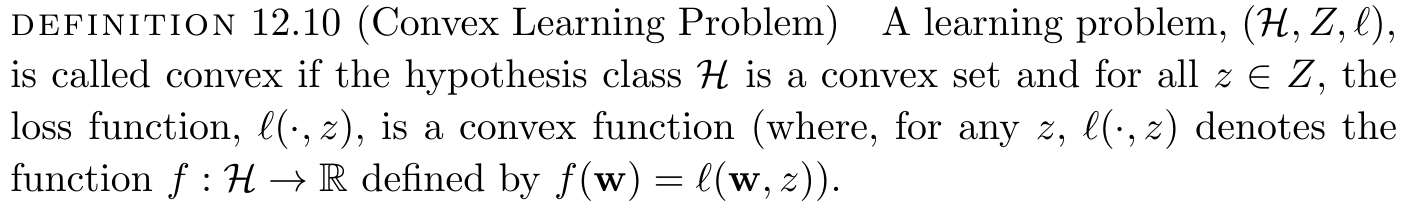
\includegraphics[scale=0.3]{def_12_10}
\end{figure}

\end{frame}

\begin{frame}
\frametitle{Convex Learning Problems: Intro}

\begin{figure}
    \centering
    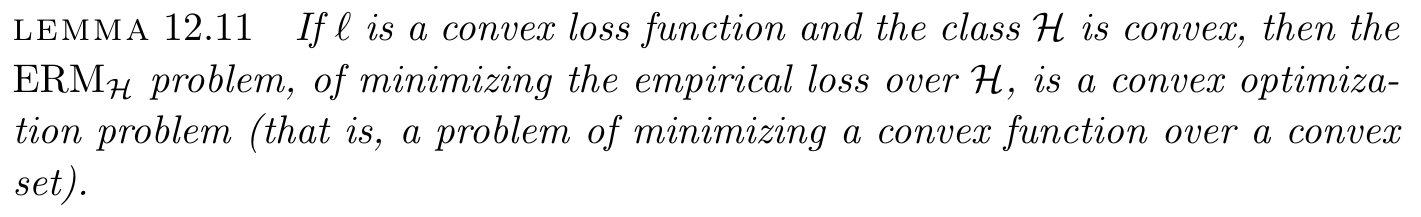
\includegraphics[scale=0.3]{lemma_12_11}
\end{figure}

Example 12.7 (Linear Regression with the Squared Loss)

\end{frame}

\begin{frame}
\frametitle{Convex Learning Problems: Learnability}
\begin{itemize}
    \item is convexity a sufficient condition for the learnability of a problem?
    \item are all convex learning problems over $R^d$ learnable?
\end{itemize}

ANS:\\
Not all convex learning problems over Rd are learnable.

Convex problems are learnable under some additional restricting conditions:\\
the properties of convexity, boundedness, and Lipschitzness or smoothness of the
loss function are sufficient for learnability.

\end{frame}

\begin{frame}
\frametitle{Convex Learning Problems: Learnability}
TWO families of learning problems are learnable.

\begin{figure}
    \centering
    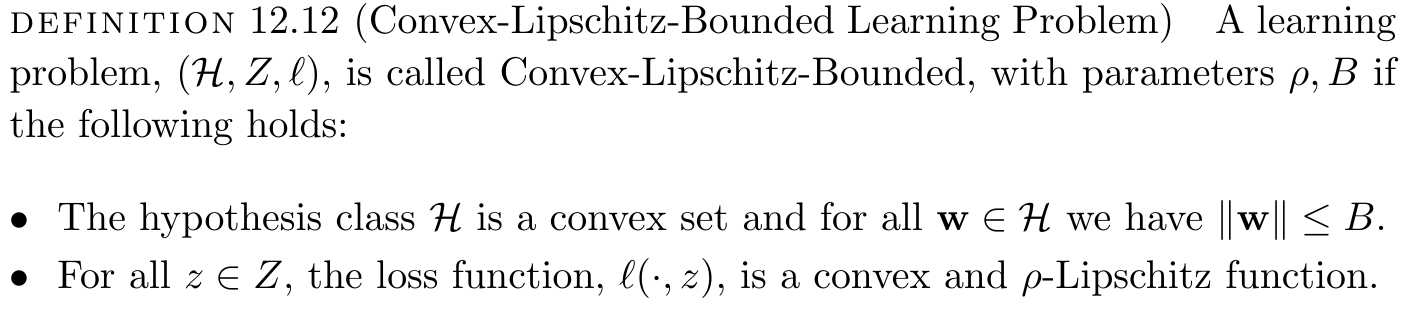
\includegraphics[scale=0.3]{def_12_12}
\end{figure}

\begin{figure}
    \centering
    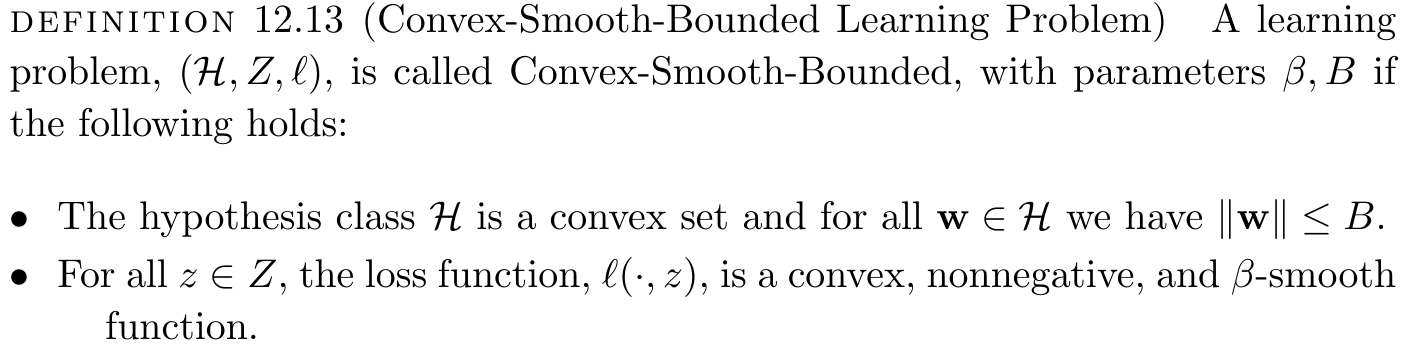
\includegraphics[scale=0.3]{def_12_13}
\end{figure}

\end{frame}


